% Chapter Template

\chapter{Results and Discussion} % Main chapter title

\label{Chapter5} % Change X to a consecutive number; for referencing this chapter elsewhere, use \ref{ChapterX}

%----------------------------------------------------------------------------------------
%	SECTION 1   % TARGET 750 WORDS IN THIS CHAPTER
%----------------------------------------------------------------------------------------

\section{Overview}
In this chapter, the results of the last chapter will be examined and discussed, covering what worked well and what could have been done differently.
The content discussed in this chapter refers only to what has been achieved in this project; a reflection on the outcome.
This is separate from the final concluding chapter which reviews the research questions, contributions to the field and covers future endeavours into the project.

%----------------------------------------------------------------------------------------
%	SECTION 2
%----------------------------------------------------------------------------------------

\section{MEGAphone Chassis/Case First Revision}
This section discusses the outcome of the final 3D-printed prototype (view chapter \ref{FinalPrint}), including what worked well and what changes might benefit the project.
Some of these changes include completed CAD designs, showing how the next print might look and are presented in the relevant figures.
The following content can be considered a critical appraisal of the final prototype.

% %-----------------------------------
% %	SUBSECTION 1
% %-----------------------------------
\subsection{Solar Panel}

The available space for the solar cell array is still seen as efficient given the available space of the device.
One major consideration that was made in retrospect was to consider an overhang for solar panels to be mounted without sticking them down as previously discussed in chapter \ref{Solar Cells}.
A 5mm overhang with 2.5mm clearance was adapted to the design with an opening at the 'top' to slide a single proprietary solar panel of the dimensions 150x125mm accounting for a theoretical 6mm overhang on all ends of the panel, leaving the exposed dimensions of 144x119mm.

\begin{figure} [h]
    \centering
    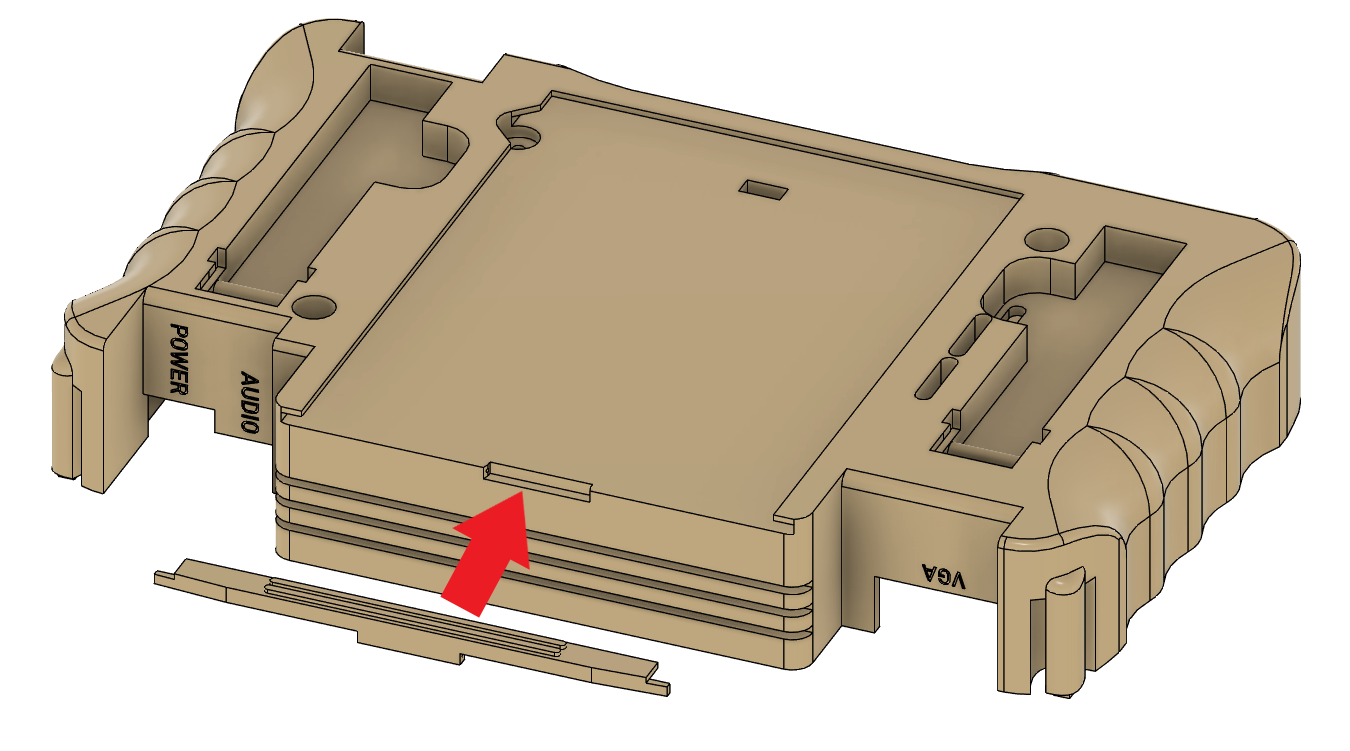
\includegraphics[width=10cm,height=10cm,keepaspectratio]{Figures/solar_new.png}
    \caption{This is a CAD model of the new housing for a solar panel, with 2.5mm clearance and 5mm overhang.}
    \label{fig:NewSolar}
    \end{figure}

This would all be contained with a separate component that slides in and snaps into place using two 'half-sphere' mechanisms that interface together.
It is however recommended that a future iteration looks at a more functional and permanent interfacing solution to this feature.

% %-----------------------------------
% %	SUBSECTION 2
% %-----------------------------------
\subsection{Battery} \label{New Battery}

While the battery housing was suitably placed and clearly labelled, attention was brought to how the battery might be secured into the housing as this had not been properly thought of before.
The proposed solution to this would be to implement a velcro strap that can be used indefinitely to secure the battery in place without any permanent modification to said battery.
As the battery is of the lithium-ion variety, it is best to avoid sticking the battery down as this can increase the risk of tearing.
Modern smartphone manufacturers tend to use their own 'glue' like substance to hold batteries in place, however, this is almost always a one time use feature.

\begin{figure} [h]
    \centering
    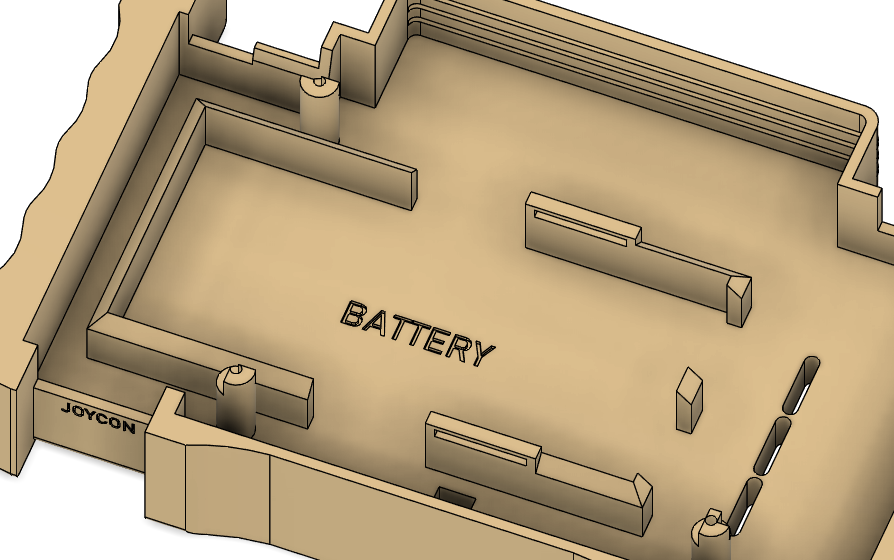
\includegraphics[width=10cm,height=10cm,keepaspectratio]{Figures/battery_new.png}
    \caption{The new considerations for the battery housing is illustrated in this figure which includes space for gripping the battery, velcro strap housing and a flush surface.}
    \label{fig:NewBatteryHousing}
\end{figure}

The method of battery removal was another aspect considered after observing the physical prototype.
Lithium-ion batteries tend to last at least a couple of years, making the event of a replacement less than frequent.
However, despite this, an avenue was seen to make battery removal easier while reducing printing material as a positive by-effect.
By making an opening on the housing for either side of the battery, two fingers would be able to help lift the battery out from the sealed surface instead of by the battery contacts.

This accounts for the placement of PCB mounting points and therefore ensures that those mounts do not obstruct the placement of this feature.
Another modification to note is that the rest of the bottom interior of the MEGAphone chassis was made flush with the battery housing to reclaim some materials and thereby reduce weight as the last 3D-print of this component is over 300g.

% %-----------------------------------
% %	SUBSECTION 3
% %-----------------------------------
\subsection{Device Stand}

Originally, the approach was to just have gravity extend the stand down when the user unlocks the mechanism, with the intent to prop the device up.

\begin{figure} [h]
    \centering
    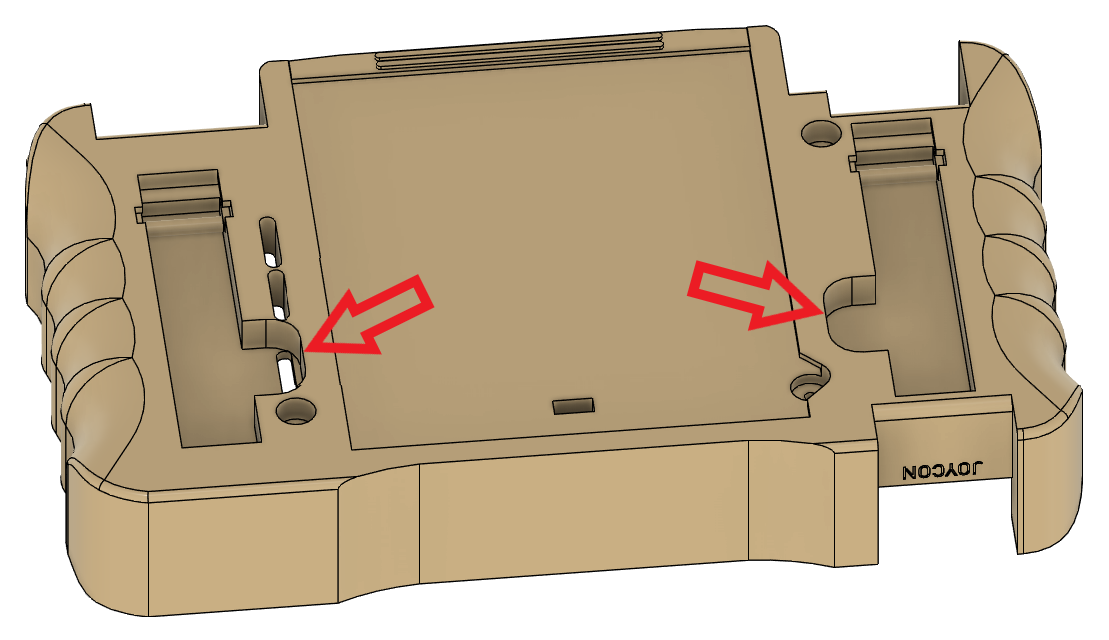
\includegraphics[width=10cm,height=10cm,keepaspectratio]{Figures/stand_new.png}
    \caption{The arched access to the stand is a new CAD consideration.}
    \label{fig:NewStand}
\end{figure}

After seeing it in practice, it was decided that implementing an arched opening would allow a finger to get a better grip on the stand to 'prop it up', independently of gravity.
Future work might include making this feature look more presentable along with a permanent hinge locking feature, however, the details of this, are discussed in chapter \ref{FutureHousing}.

%----------------------------------------------------------------------------------------
%	SECTION 3
%----------------------------------------------------------------------------------------

\section{Summary}
This chapter provides a critical appraisal of the outcome of this project.
Alterations to the project are presented, along with justifications as to why those alterations were made.
Future recommendations are also in-part provided, however, this is discussed in detail in the next chapter.